%\section{Simulation Study}

\begin{figure}[h]
    \centering
    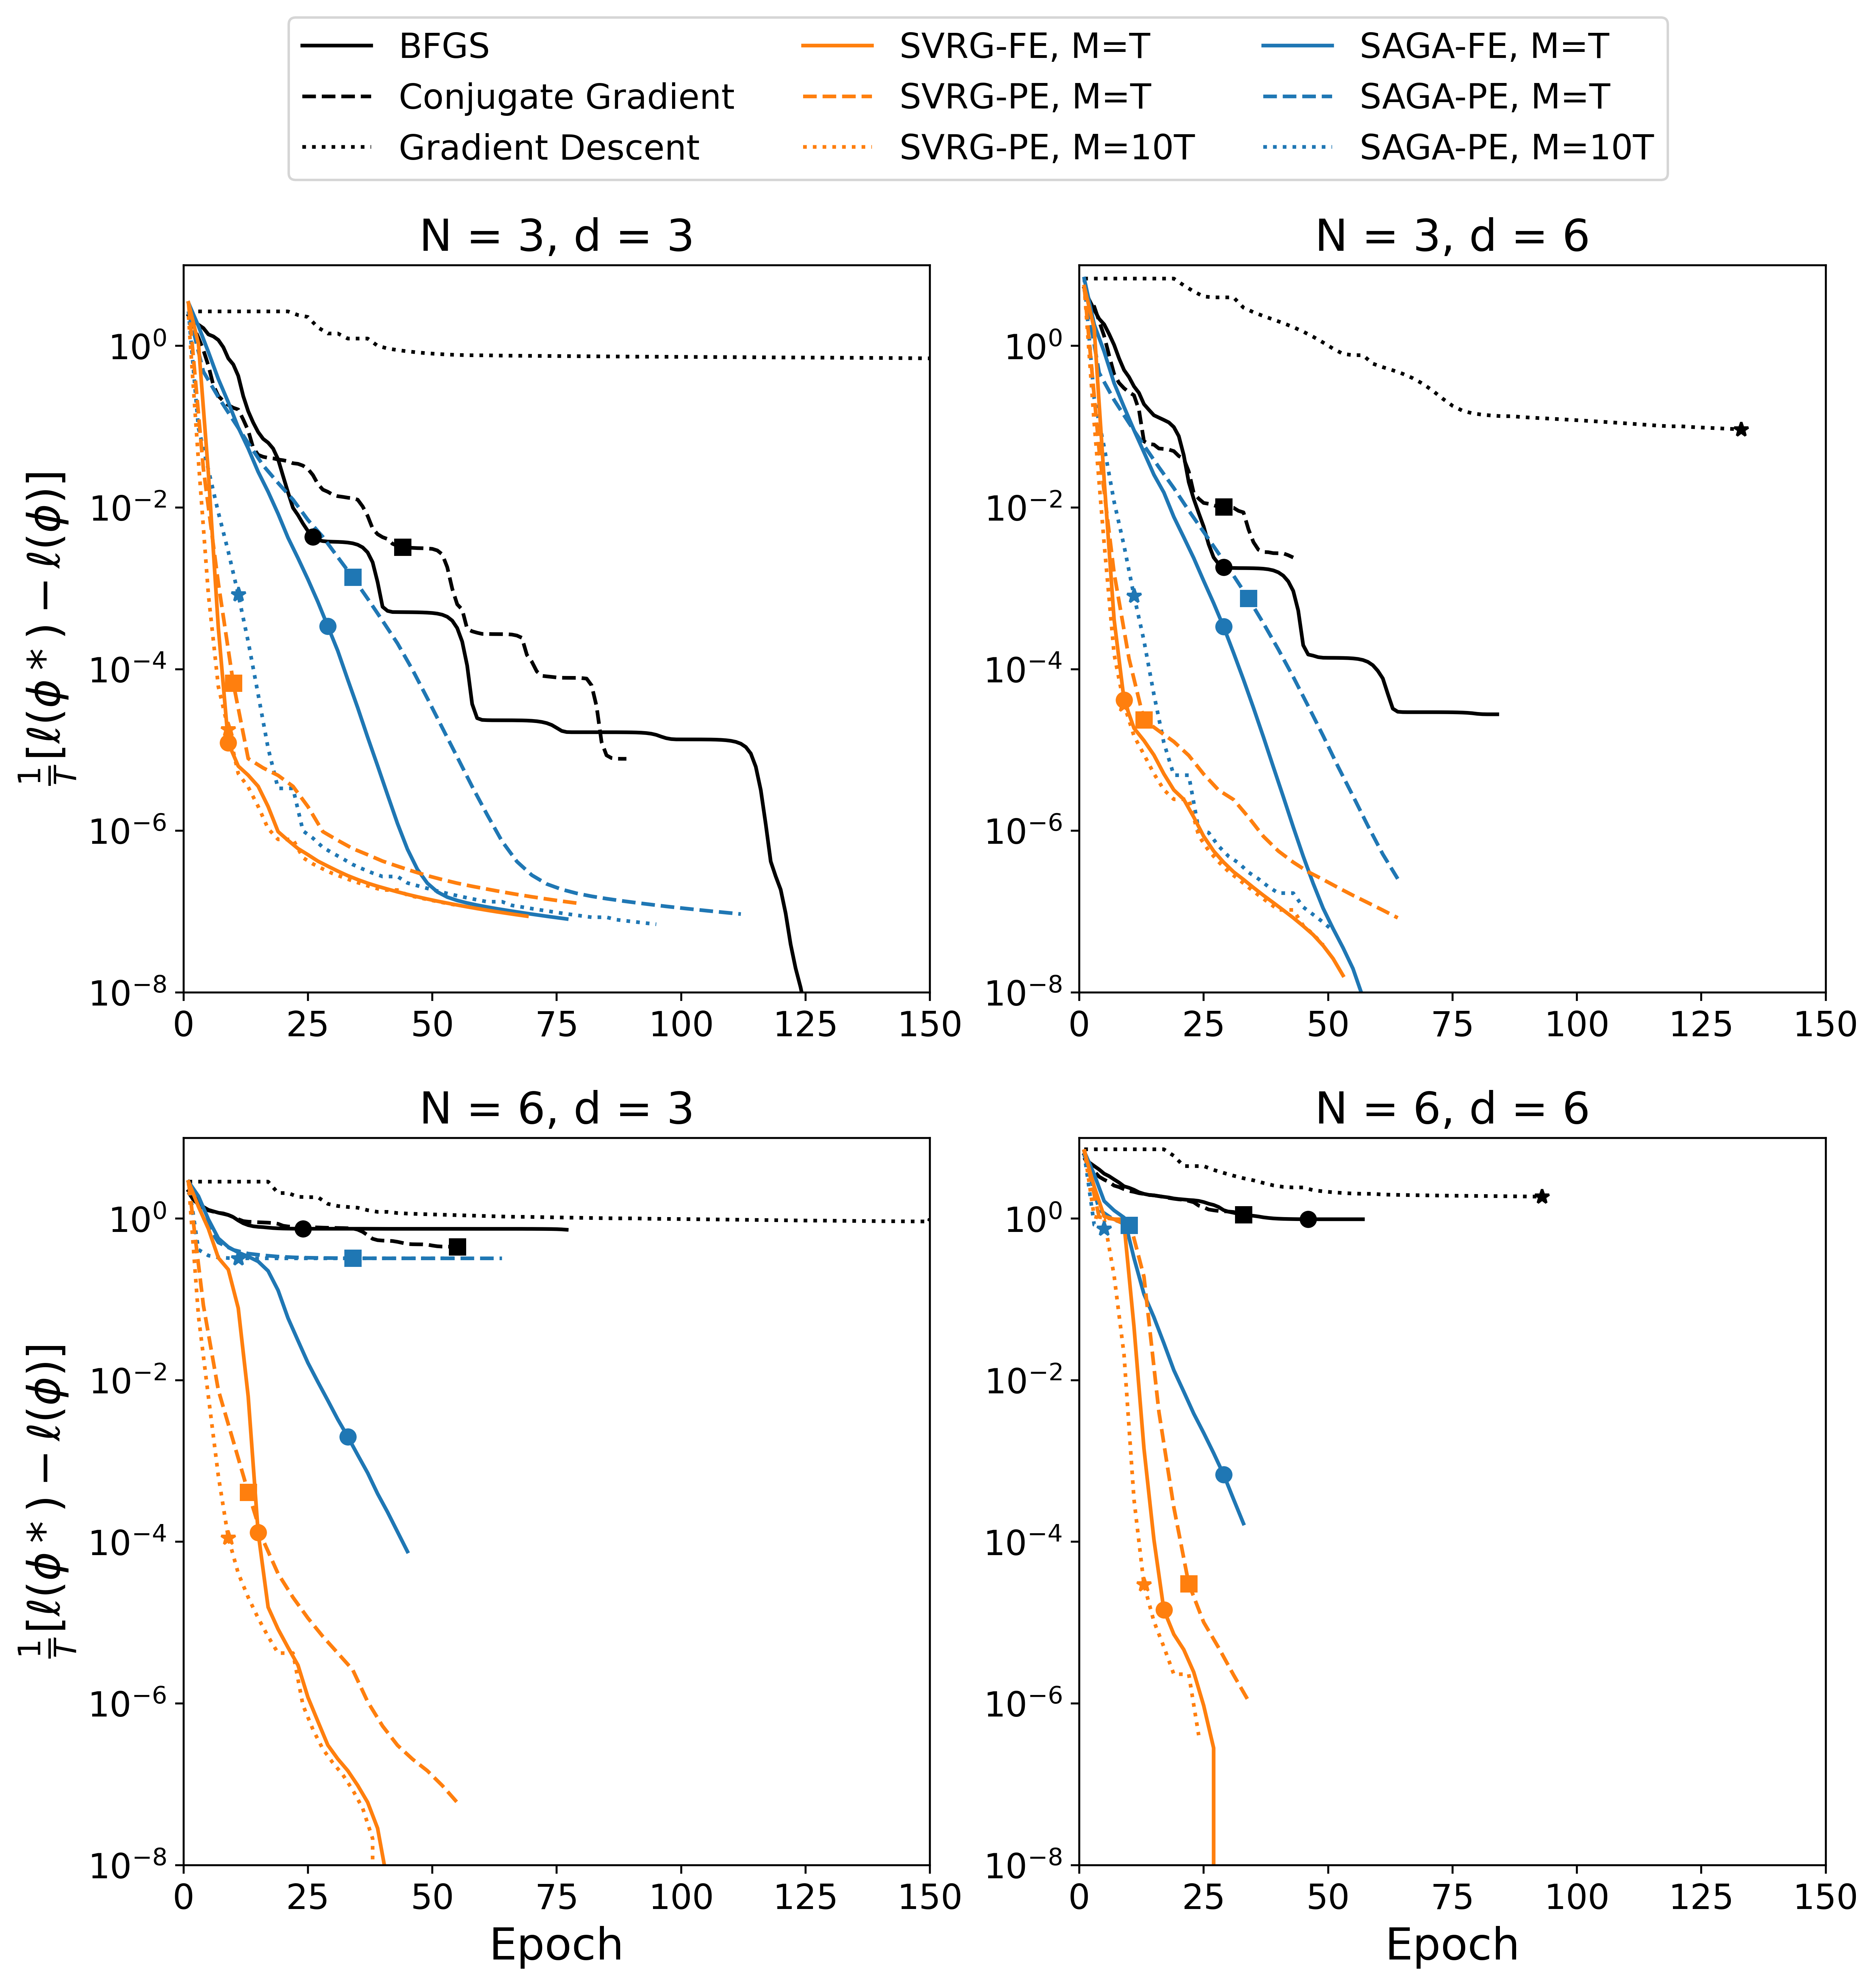
\includegraphics[width=5in]{../plt/log-like_v_epoch_T-100000-000.png}
    \caption{log-likelihood of the maximum log-likelihood minus the log-likelihood (all divided by $T$) at each epoch of a selected run of each optimization algorithm after 12 hours or 150 epochs (whichever came first) for the first data set all experiments with $T=10^{5}$, $N \in \{3,6\}$, and $d \in \{3,6\}$. One epoch represents either one full E step, $T$ stochastic gradient evaluations within the M step, or one gradient evaluation for full-gradient algorithms. The y-axis is on a log-scale. FE corresponds to $P = \texttt{False}$, and PE corresponds to $P = \texttt{True}$. We display the random initialization of each algorithm that resulted in the highest likelihood after 12 hours. Dots correspond to the epoch and likelihood at convergence. Convergence was achieved when the gradient norm of the log-likelihood (divided by $T$) was less than $10^{-2}$. The tolerance was set to $10^{-2}$ because it was the lowest tolerance that all algorithms regularly converged to within 12 hours.}
    \label{fig:ll_trace_sim}
\end{figure}
%
\begin{figure}[h]
    \centering
    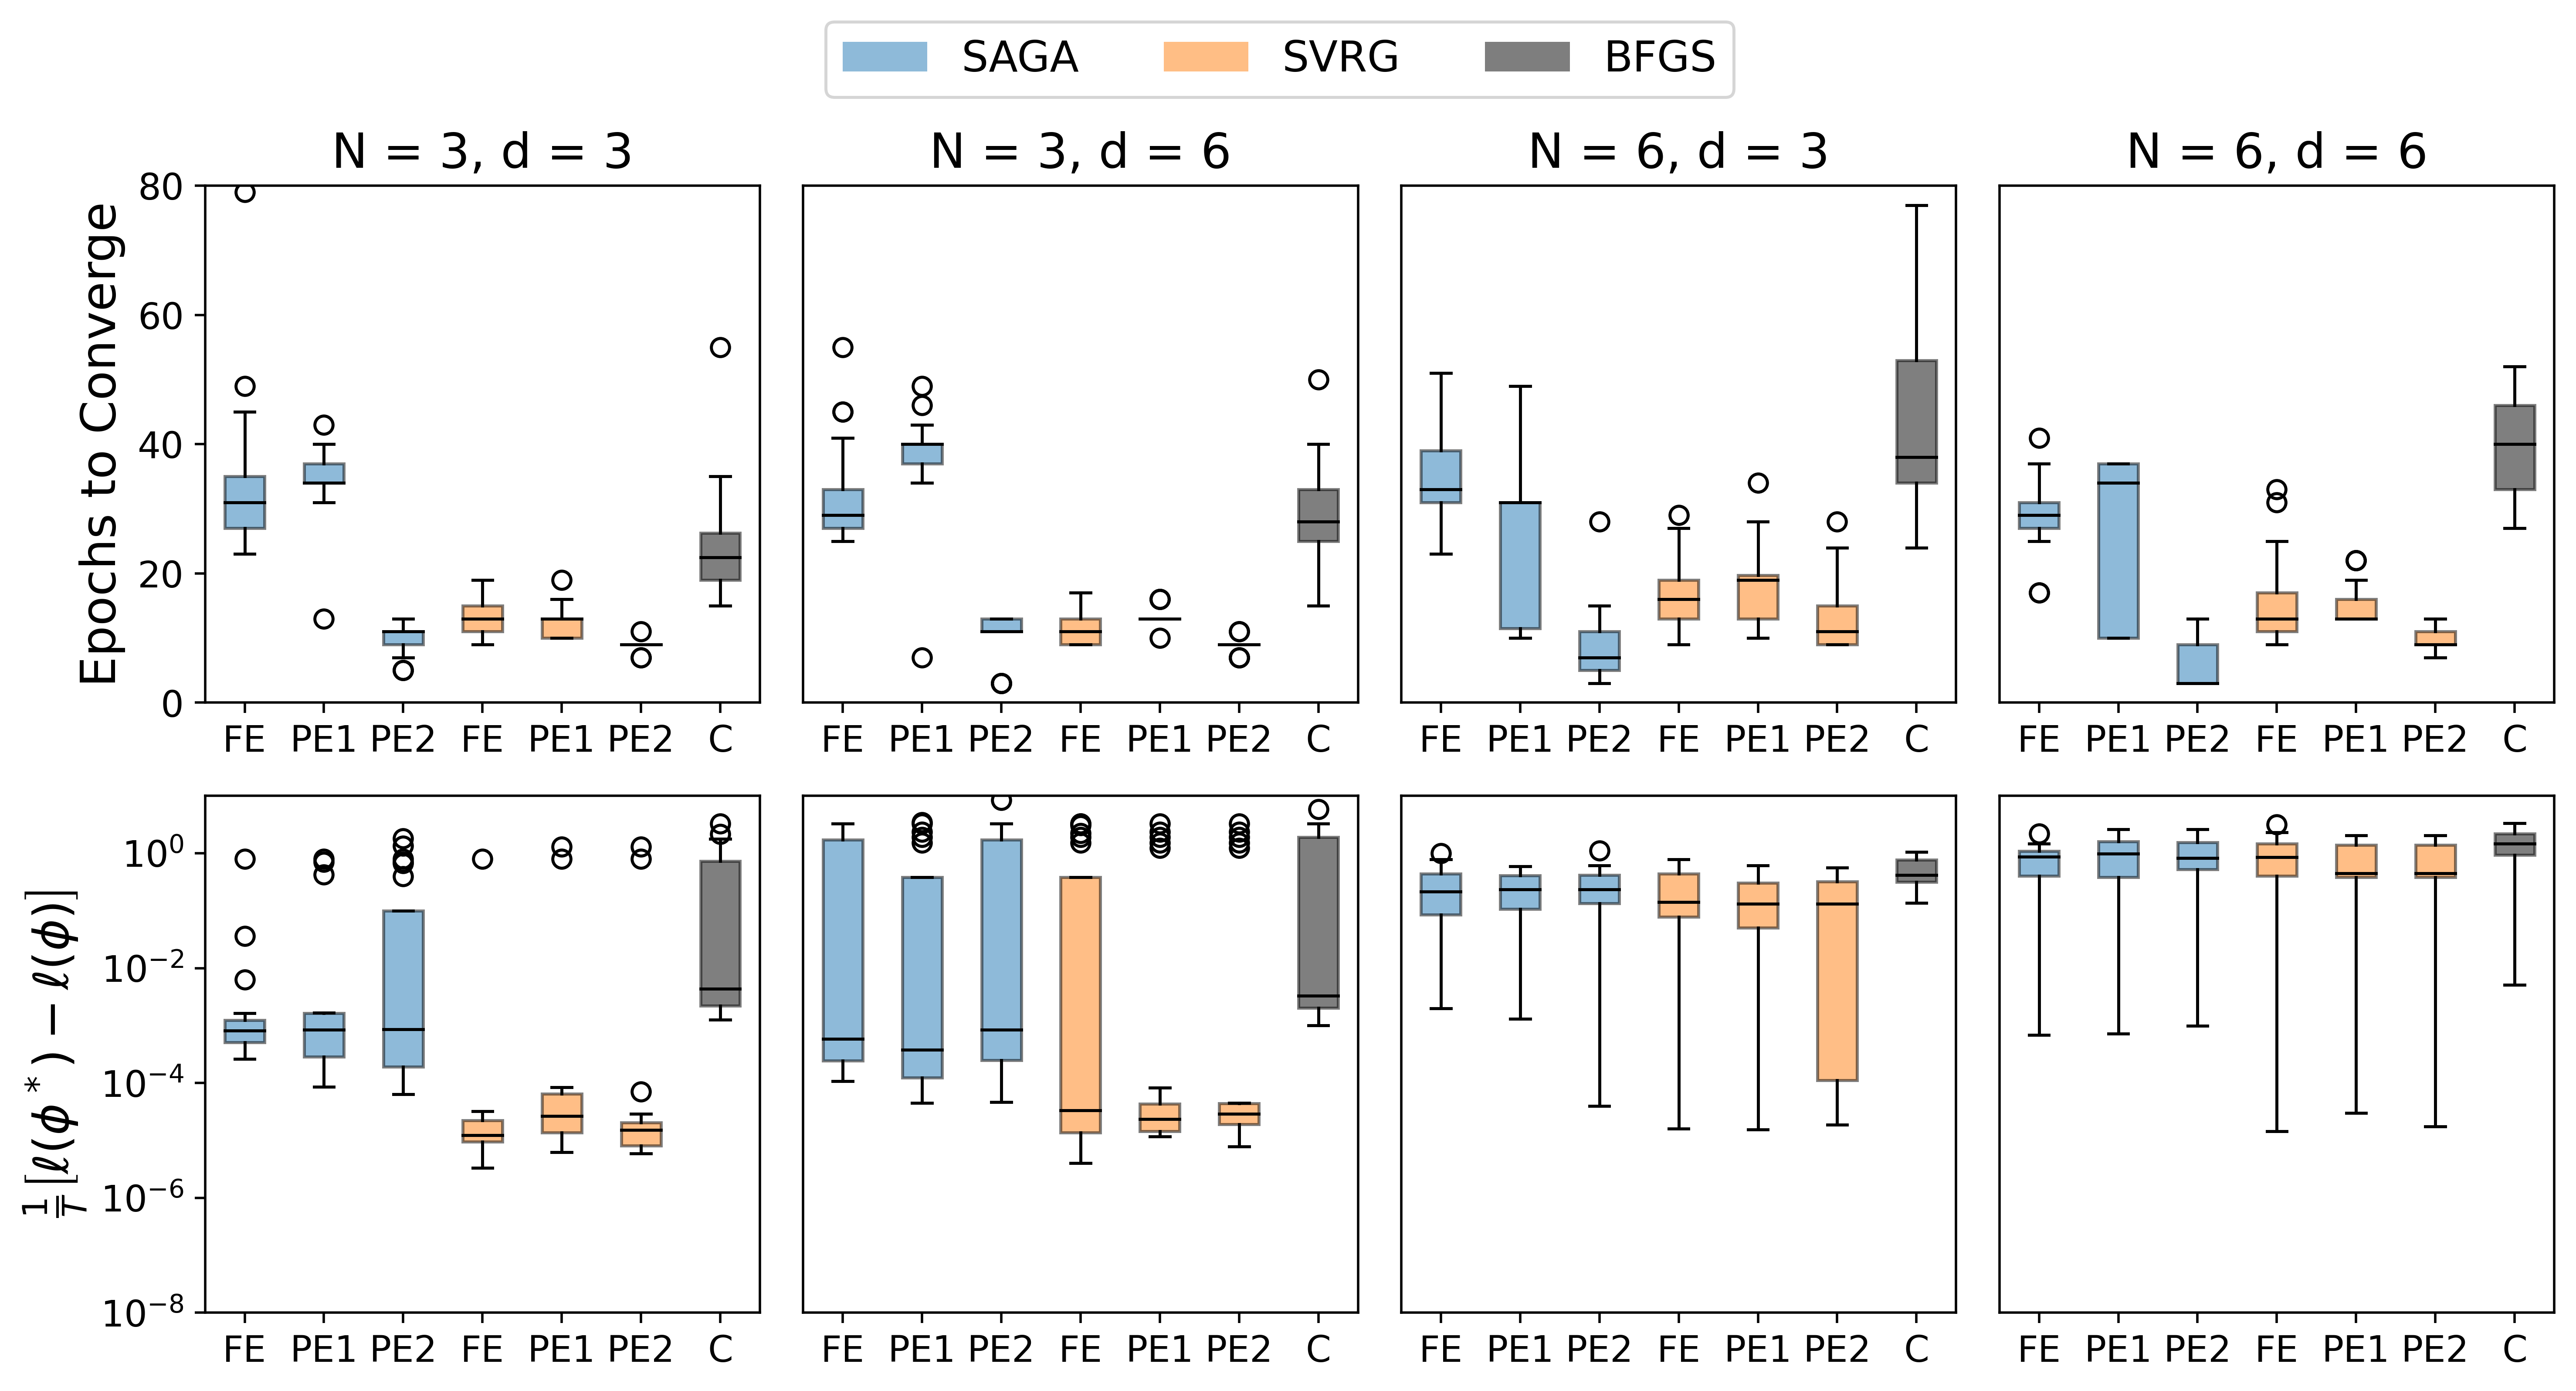
\includegraphics[width=6in]{../plt/boxplots_sim_T_100000.png}
    \caption{Box plots showing epochs to converge (top) and the log-likelihood of the maximum log-likelihood minus the log-likelihood (all divided by $T$) at convergence (bottom) for each optimization algorithm. Unlike Figure (\ref{fig:ll_trace_sim}), results are displayed for all algorithms, data sets, and initial parameter values. FE corresponds to $\{P = \texttt{False}, M = T\}$, PE1 corresponds to $\{P = \texttt{True}, M = T\}$, and PE2 corresponds to $\{P = \texttt{False}, M = 10T\}$. Blue corresponds to SAGA and orange corresponds to SVRG. Results are shown for all simulation studies with $T=10^{5}$, $N=3$ and $d=3$ (left), $N=3$ and $d=6$ (left-middle), $N=6$ and $d=3$ (right-middle), and $N=6$ and $d=6$ (right). One epoch represents either one full E step, $T$ iterations with the M step, or one gradient step for full-gradient algorithms. The y-axis of the bottom row is on a log-scale.}
    \label{fig:boxplots_sim}
\end{figure}
%
\begin{figure}[h]
    \centering
    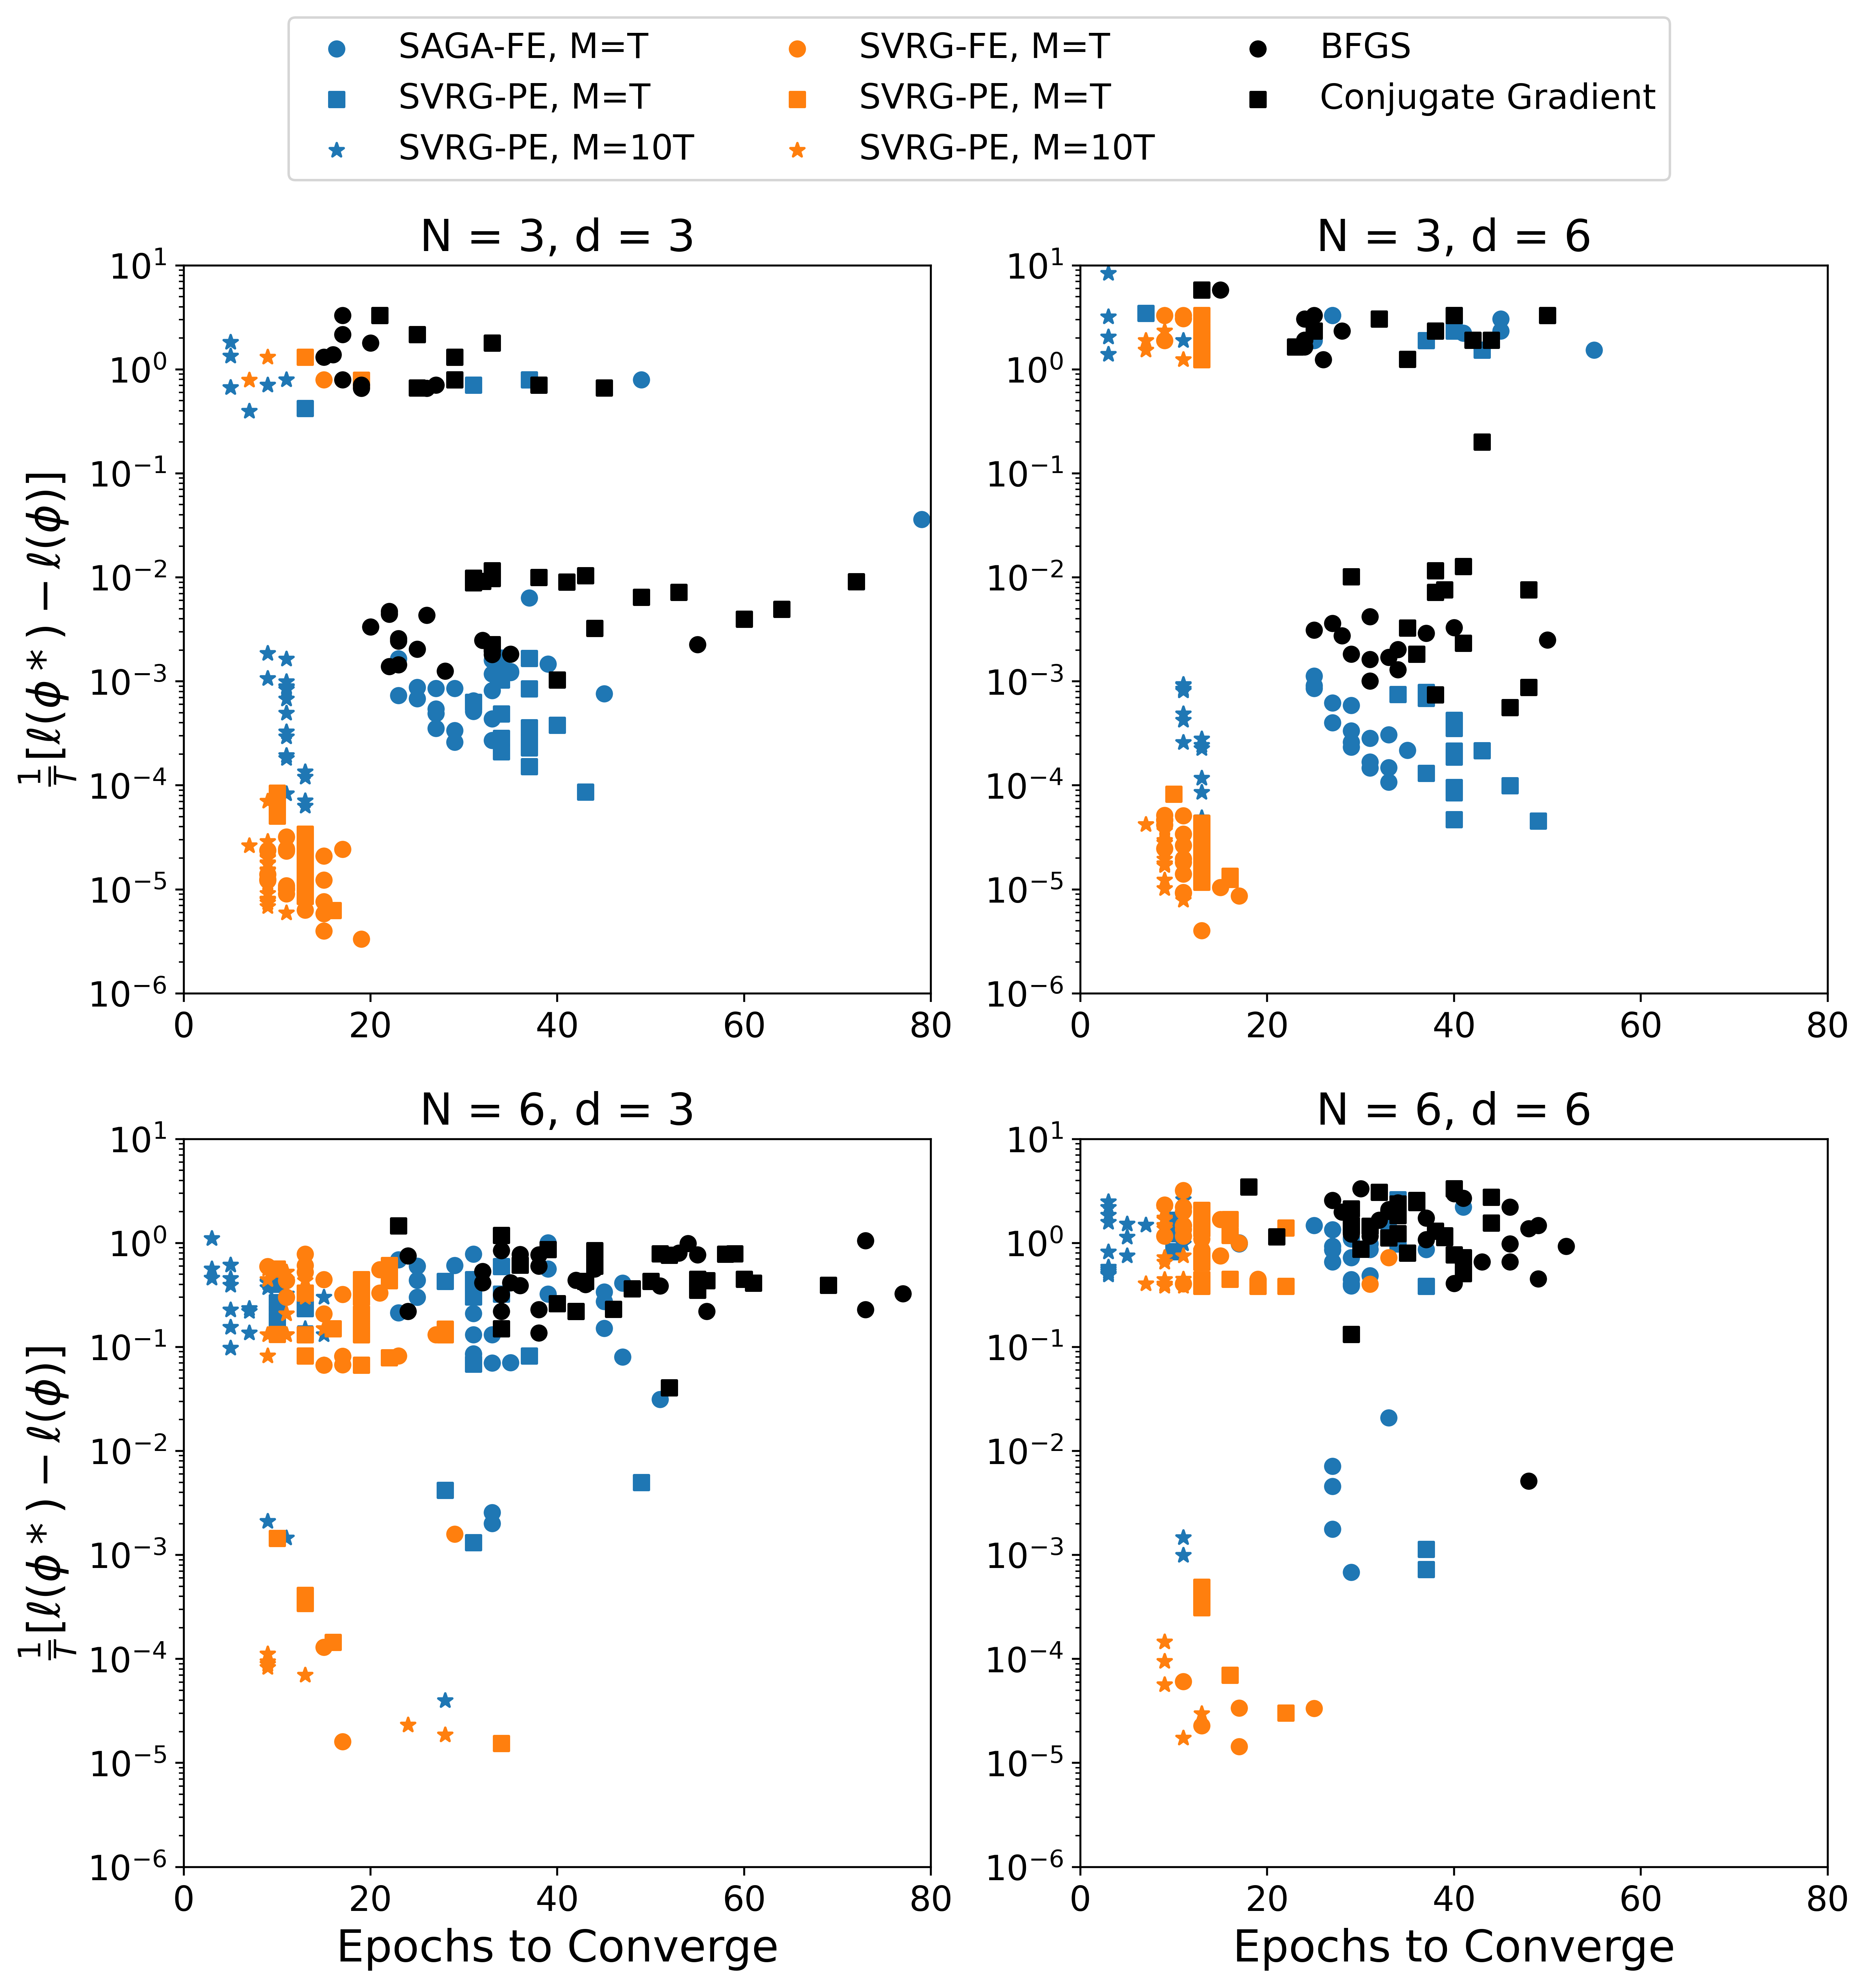
\includegraphics[width=5in]{../plt/scatter_sim_T_100000.png}
    \caption{Log-likelihood of the maximum log-likelihood minus the log-likelihood (all divided by $T$) at convergence versus epochs to converge for all simulation studies with $T=10^{5}$, $N=3$ and $d=3$ (top left), $N=3$ and $d=6$ (top right), $N=6$ and $d=3$ (bottom left), and $N=6$ and $d=6$ (bottom left). One epoch represents either one full E step, $T$ iterations with the M step, or one gradient step for full-gradient algorithms. The y-axis is on a log-scale.}
    \label{fig:scatter_sim}
\end{figure}

\subsection{Simulation Procedure}

To test the performance of Algorithm (\ref{alg:EM-VRSO}), we ran eight simulation experiments. For a given experiment, we simulated $T \in \{10^3,10^5\}$ observations from an HMM with $N \in \{3,6\}$ hidden states and observations $y_t \in \bbR^d$, with $d \in \{3,6\}$. All possible combinations of $T$, $N$, and $d$ comprised a total of $2^3 = 8$ experiments. For each experiment, we simulated five data sets. For every experiment and data set, $Y_t \mid X_t = i$ followed a normal distribution with mean $\mu^{(i)}$ and covariance matrix $\bfSigma^{(i)}$, $\calN(\mu^{(i)},\bfSigma^{(i)})$. We defined $\mu^{(i)}$ and $\bfSigma^{(i)}$ for every data set as
%
%\begin{equation}
$\mu^{(i)} \sim \calN(0,I)$ and $\bfSigma^{(i)} = \text{diag}(\exp(-2))$ for $i \in \{1,\ldots,N\}$
%\end{equation}
%
where $I$ is the identity matrix.
%
We set the transition probability matrices of the generating process to depend upon $T$ to keep the expected number of total transitions at 100. This simulates sequences of observations that are sampled at either low- or high- frequencies.
%
Denote the true transition probability matrix from an experiment with $T$ observations and $N$ hidden states as $\bfGamma_{T,N}$. We set $\bfGamma_{10^3,3} \in \bbR^{3 \times 3}$ with diagonal elements of 0.9 and off-diagonal elements of 0.05, $\bfGamma_{10^3,6} \in \bbR^{6 \times 6}$ with diagonal elements of 0.9 and off-diagonal elements of 0.02, $\bfGamma_{10^5,3} \in \bbR^{3 \times 3}$ with diagonal elements of 0.999 and off-diagonal elements of $5 \times 10^{-4}$. and $\bfGamma_{10^3,6} \in \bbR^{6 \times 6}$ with diagonal elements of 0.999 and off-diagonal elements of $2 \times 10^{-4}$. 
%
\iffalse
\begin{gather*}
    \bfGamma_{10^3,3} = 
    \begin{pmatrix} 
        0.9 & 0.05 & 0.05 \\
        0.05 & 0.9 & 0.05 \\
        0.05 & 0.05 & 0.9
    \end{pmatrix},
    \qquad
    \bfGamma_{10^3,6} = 
    \begin{pmatrix} 
        0.9  & 0.02 & 0.02 & 0.02 & 0.02 & 0.02 \\
        0.02 & 0.9  & 0.02 & 0.02 & 0.02 & 0.02 \\
        0.02 & 0.02 & 0.9  & 0.02 & 0.02 & 0.02 \\
        0.02 & 0.02 & 0.02 & 0.9  & 0.02 & 0.02 \\
        0.02 & 0.02 & 0.02 & 0.02 & 0.9  & 0.02 \\
        0.02 & 0.02 & 0.02 & 0.02 & 0.02 & 0.9  \\
    \end{pmatrix},
    \\
    \bfGamma_{10^5,3} = 
    \begin{pmatrix} 
        0.999 & 0.0005 & 0.0005 \\
        0.0005 & 0.999 & 0.0005 \\
        0.0005 & 0.0005 & 0.999
    \end{pmatrix}
    \qquad
    \bfGamma_{10^5,6} = 
    \begin{pmatrix} 
        0.999  & 0.0002 & 0.0002 & 0.0002 & 0.0002 & 0.0002 \\
        0.0002 & 0.999  & 0.0002 & 0.0002 & 0.0002 & 0.0002 \\
        0.0002 & 0.0002 & 0.999  & 0.0002 & 0.0002 & 0.0002 \\
        0.0002 & 0.0002 & 0.0002 & 0.999  & 0.0002 & 0.0002 \\
        0.0002 & 0.0002 & 0.0002 & 0.0002 & 0.999  & 0.0002 \\
        0.0002 & 0.0002 & 0.0002 & 0.0002 & 0.0002 & 0.999  \\
    \end{pmatrix}.
\end{gather*}
\fi
%
We randomly defined the initial distribution as $\bfdelta \sim \text{dir}(\onevec_N)$ for every experiment and data set.

\subsection{Optimization Procedure}

We estimated the parameters of the generating model for all five data sets and all eight experiments using six different versions of Algorithm (\ref{alg:EM-VRSO}). In particular, we used $A \in \{\text{SVRG, SAGA}\}$, and for each value of $A$, we used the combinations $\{P = \texttt{False}, ~ M = T\}$, $\{P = \texttt{True}, ~ M = T\}$, and $\{P = \texttt{True}, ~ M = 10T\}$. Recall that setting $P = \texttt{True}$ corresponds to integrating a partial E step into the variance-reduced stochastic M step. The variable $M$ corresponds to the number of iterations of SAGA or SVRG that are performed at each M step of the algorithm. It is natural to set $M=T$ to approximately balance the computational load of the E step and the M step. Nonetheless, we run $M=10T, P = \texttt{True}$ to test the algorithm when the majority of the computational load is placed on the combined partial E / stochastic M step. We also estimated the HMM parameters using three baseline methods: BFGS \citep{Fletcher:2000}, the conjugate gradient method \citep{Fletcher:1964}, and full-batch gradient descent. All baselines were implemented using the Scipy library in Python \citep{Virtanen:2019}.

We sampled a total of five random parameter initializations for each data set / experiment pair, and then ran all nine optimization algorithms on every parameter initialization. Each parameter initialization was re-used for each algorithm to ensure consistency between optimization algorithms. Let $\bar y$ denote the sample mean and $\bfQ$ denote the sample covariance of the observation sequence $\{y_t\}_{t=1}^T$. We initialized $\bftheta_0$ and $\bfeta_0$ as

\begin{gather*}
    \mu^{(i)}_0 \sim \calN(\bar y, \text{diag}(\bfQ)), \quad \bfSigma^{(i)}_0 = \text{diag}(\bfQ), \qquad i \in \{1,\ldots,N\}, \\
    %
    \eta^{(i)}_0 \sim \calN(0,1), \qquad i = 2,\ldots,N \\
    %
    \eta^{(i,j)}_0 \sim \calN(-2,2^2), \qquad i,j = 1,\ldots,N, \quad i \neq j.
\end{gather*}
%
%If the 2-norm of the average estimated gradient $||\frac{1}{T}\sum_{t=1}^T \widehat \nabla F^{(k,m)}_t + \widehat \nabla G^{(k,m)}_t||$ ever fell below a tolerance of $10^{-8}$, we terminated the M step of algorithm and moved on to the E step. Likewise, if the relative change of the log-likelihood after one full E  and M  step of the EM algorithm ever fell below a tolerance of $10^{-10}$, we terminated the algorithm altogether. We found the ground truth MLEs by running the traditional EM algorithm until the relative change in the log-likelihood was on the order of machine precision $10^{-15}$.

Throughout the optimization procedure, we assumed that $\bfSigma^{(i)}$ was diagonal for all $i \in \{1,\ldots,N\}$, which is in line with the generating model described above. Further, because $\bfSigma^{(i)}$ must have positive diagonal elements, we parameterized $\bfSigma^{(i)}$ as 
%
\begin{equation}
    \bfSigma^{(i)} = 
    \begin{pmatrix}
        \exp(\rho_1)^2 & 0 & \ldots & 0 \\
        0 & \exp(\rho_2)^2 & \ldots & 0 \\
        \vdots & \vdots & \ddots & \vdots \\
        0 & 0 & \ldots & \exp(\rho_N)^2 \\
    \end{pmatrix},
\end{equation}
%
and performed inference on $\boldsymbol{\rho} = \begin{pmatrix} \rho_1 & \ldots & \rho_N \end{pmatrix}$, which is unconstrained.

All six algorithms were initialized with step sizes of $\lambda_{\bftheta} = 1/3 \hat L_G$ and $\lambda_{\bfeta} = 1/3 \hat L_H$. The Lipschitz constants were initialized as $\hat L_G = \hat L_H = 100/3$ and updated during the optimization routine according to the procedure from section \ref{subsec:est_L}. 
%
All algorithms and baselines were run for a total of 12 hours on the Compute Canada Cedar cluster on nodes with 16GB of RAM.

\subsection{Simulation Results}

Algorithm (\ref{alg:EM-VRSO}) with $A=\text{SVRG}$ significantly sped up the optimization procedure, as it usually converged in at most half as many epochs compared to the baselines for each experiment (see Figures (\ref{fig:ll_trace_sim} - \ref{fig:scatter_sim})). Algorithm (\ref{alg:EM-VRSO}) with $A=\text{SAGA}$ also tended to converge faster than the baselines for all experiments except for those with $N=3$. Algorithm (\ref{alg:EM-VRSO}) with $A=\text{SAGA}$ also converged in significantly fewer epochs when $P = \texttt{True}$ and $M=10T$. 
%
All methods were prone to converge to local minima, especially when $N=6$, when the likelihood surface is highly multi-modal. However, Algorithm (\ref{alg:EM-VRSO}) tended to converge to areas of higher likelihood than the baseline for almost all experiments. The sole exception was when $T=10^3$, $N=6$, and $d=6$, where BFGS and the conjugate gradient method were less likely to get stuck in local minima (See Figures (1--2) in Supplement A). However, that experiment is a small-data setting, and we are primarily interested in modelling very large data sets. %This indicates that in a high-dimensional, small-data setting, our methods may have diminishing returns. However, our intention in this paper is to improve inference in big-data settings. 
%
%Our methods tend to converge to areas of likelihood at least as high as the baselines for all experiments with the exception of those with $T=10^{3}$ and $N=6$, where BFGS achieves the highest log-likelihood after approximately 120 epochs (See Supplement A).
%
We present figures analogous to Figure (\ref{fig:ll_trace_sim}) for all five data sets corresponding to all experiments in Supplement A. All figures associated experiments where $T=10^3$ can also be found in Supplement A. 

%The algorithms which implement a partial E step appear to help the algorithm move to areas of high likelihood, especially within the first ~20 epochs of optimization. We show zoomed in versions of Figure (\ref{fig:ll_trace_sim}) in the appendix to highlight the advantages of the partial E step early in the optimization procedure.
%
%Overall, SVRG appears to converge faster than SAGA for all algorithms. 
%This may be a function of our step size ($1/3 \hat L$), but that step size was selected based upon suggestions from the SAGA paper \citep{Defazio:2014}. 


%The partial E  step within Algorithm (3) looks to help primarily for experiments with $N=6$, especially for early epochs of the algorithm. This makes sense since the weights from the EM algorithm will be out of date quickly when the parameter estimates are poor early in the EM algorithm.

%SAGA without a partial E step performs similarly to the EM algorithm in a per-epoch basis because SAGA is successfully converging for the M step when $M = T$. However, it does not perform as well as the EM algorithm on a per-time basis because the M step is significantly slower when using SAGA vs the closed-form solution. This behavior is expected, and SAGA has a significant advantage over the EM algorithm in that it only requires gradients rather than sufficient statistics.

%mplementing a partial E step shows that SAGA can outperform the EM algorithm when the parameter estimates are far from the optimal solutions and when the underlying HMM does not mix rapidly. This is likely because the weights of the $F$ and $G$ are very inaccurate at first, and updating them early in the optimization procedure yields a significant speed-up. In addition, if the Markov chain is rapidly mixing, then updates to $\gamma_{t_m}$ and $\xi_{t_m}$ at a single data point are more accurate. Future work may involve performing the partial-E step for many weights at once sequentially, depending upon the mixing time of the current estimate of $\eta_k$.